\documentclass{beamer}
\usetheme{Copenhagen}
\usecolortheme{seahorse}
\usefonttheme[onlymath]{serif}

\usepackage{setspace}
\usepackage{xcolor}
\usepackage{graphicx}
\usepackage{multimedia}
\usepackage{fontawesome5}
\usepackage[most]{tcolorbox}
\usepackage{empheq}
\usepackage{fancybox}
\usepackage{annotate-equations}
\usepackage{tikz}
\usetikzlibrary{positioning, calc, shapes.geometric, shapes.multipart, 
	shapes, arrows.meta, arrows, 
	decorations.markings, external, trees}
\tikzstyle{Arrow} = [
thick, 
decoration={
	markings,
	mark=at position 1 with {
		\arrow[thick]{latex}
	}
}, 
shorten >= 3pt, preaction = {decorate}
]

\definecolor{teel}{HTML}{00AEB3}
\definecolor{redorange}{HTML}{F26035}
\definecolor{ForestGreen}{RGB}{34,139,34}
\definecolor{darkgreen}{HTML}{06402B}
\definecolor{CarolinaBlue}{HTML}{4B9CD3}
\usecolortheme[named=CarolinaBlue]{structure}


\title[Network-TMLE]{Estimating the risk of influenza under differing distributions of vaccination among university students}
\author[Paul Zivich]{Paul Zivich \\~\\ Assistant Professor \\ Department of Epidemiology \\ Gillings School of Global Public Health \\ University of North Carolina at Chapel Hill}

\setbeamercovered{transparent}
\setbeamertemplate{navigation symbols}{}  % gets rid of the dumb navigation symbols
\setbeamertemplate{page number in head/foot}{\insertframenumber}  % adds slide #
\setbeamertemplate{headline}{}

\AtBeginSection[]{
	\begin{frame}
		\vfill
		\centering
		\begin{beamercolorbox}[sep=8pt,center,shadow=true,rounded=true]{title}
			\usebeamerfont{title}\insertsectionhead\par%
		\end{beamercolorbox}
		\vfill
	\end{frame}
}

\begin{document}
	
\begin{frame}[plain]
	\maketitle
\end{frame}

\begin{frame}{Acknowledgements\footnote[frame]{Footnotes are for asides or references, but are fair game for questions}}
	This presentation is built from parts of my dissertation
	~\\~\\
	\textbf{Dissertation Committee}: Allison Aiello (chair), Alan Brookhart, Michael Hudgens, James Moody, David Weber \\~\\
	\textbf{Funding}: K01AI177102 (current), T32HD091058 (former), U01CK000185 (eXFLU) \\~\\
	\textbf{Disclaimer}: views (and errors) are mine and not those of NIH or colleagues \\~\\
	\begin{center}
		\small
		\faEnvelope \quad pzivich@unc.edu \qquad \quad 
		\faGithub \quad pzivich \qquad \quad
		pausalz@bsky.social
	\end{center}
\end{frame}

\begin{frame}{Influenza}
	Influenza causes substantial morbidity, mortality, economic costs 
	~\\~\\
	Influenza prevention among university students
	\begin{itemize}
		\item Elevated risk of infection, low vaccination rates, importance for further transmission\footnote[frame]{Layde et al. \textit{JID} 1980;142(3):347-352, Bednarczyk et al. \textit{Vaccine} 2015;33(14):1659-1663}
		\item A key prevention strategy is vaccination
	\end{itemize}
	~\\
	Prior research on university students has focused on
	\begin{itemize}
		\item Direct, or unit-treatment, effect of vaccination
		\item Focused on vaccination uptake as outcome
	\end{itemize}
	~\\
	Not influenza incidence under large scale changes in vaccination
\end{frame}

\begin{frame}{Motivation}
	\textbf{Question}: What would the risk of influenza infection be under plans that increase the probability of influenza vaccination uptake among university students at a midwest university from January to April 2013?
	~\\~\\
	\textbf{Data}: eX-FLU cluster randomized trial ($n=454$)\footnote[frame]{Aiello AE et al. 2016 \textit{Epidemics}; 15:38-55}
	\begin{itemize}
		\item Randomized 3-day self-isolation
		\item 10-weeks of follow-up
		\item Collected information on vaccination, risk factors for respiratory infections, respiratory infections
	\end{itemize}
\end{frame}

\begin{frame}{In-Person Contacts Between Students}
	\begin{center}
		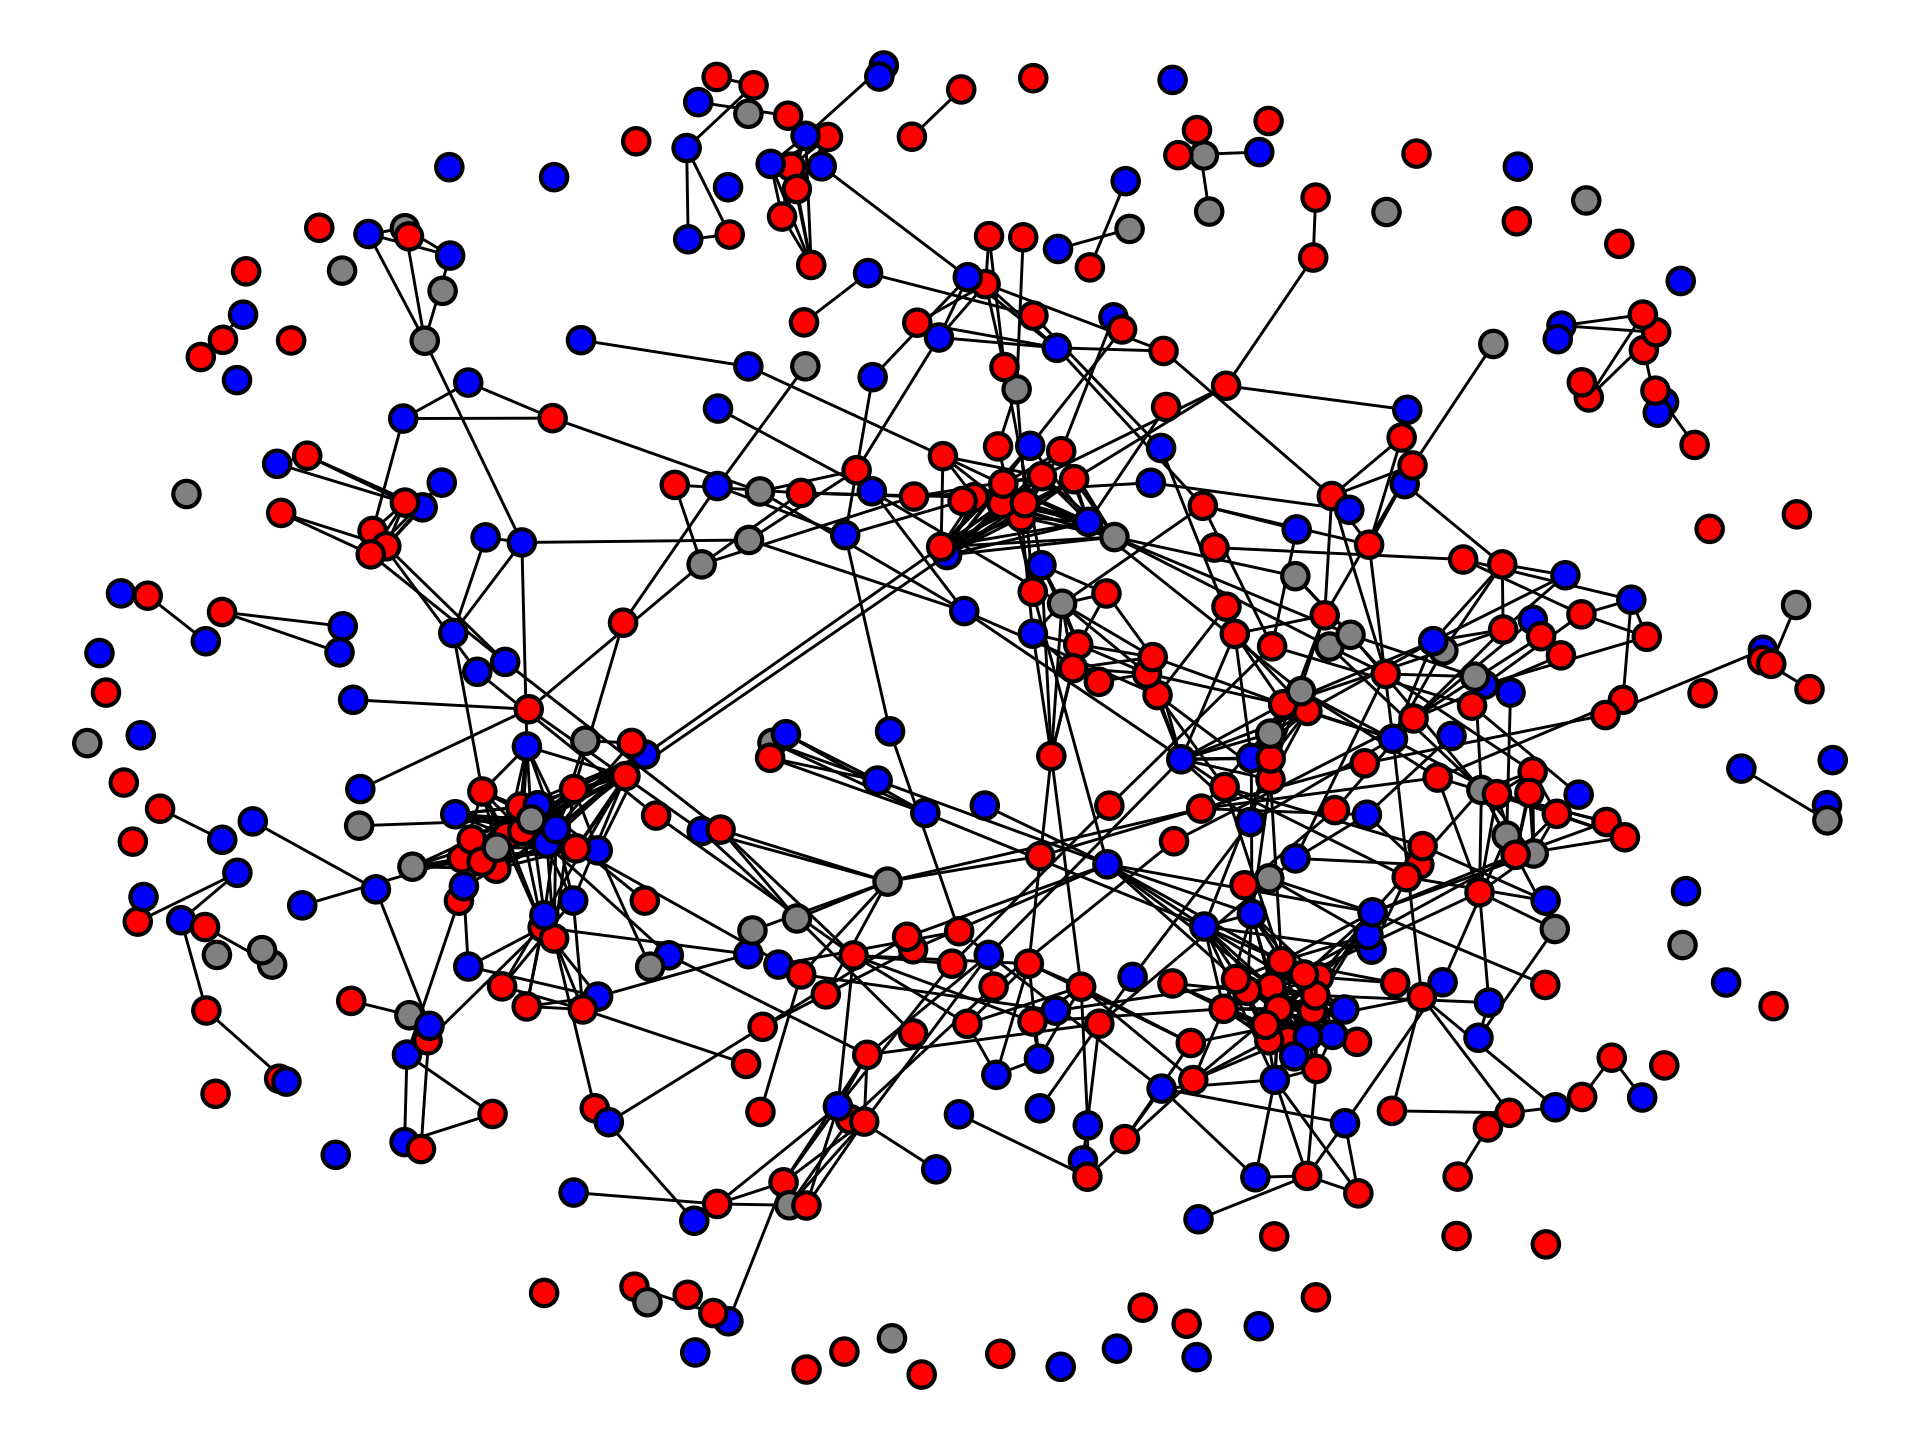
\includegraphics[width=0.95\linewidth]{images/exflu_network.png}
	\end{center}
\end{frame}

\begin{frame}{Challenges}
	\begin{itemize}
		\item[1.] Interference \& spillover effects
		\begin{itemize}
			\item Vaccination of one affects another
		\end{itemize}
		\item[2.] Missing vaccination data
		\item[3.] Measurement error of contacts
	\end{itemize}
\end{frame}

\section{Parameter}

\begin{frame}{Notation}
	$Y_i$: observed outcome (i.e., influenza infection) for unit $i$ ~\\~\\
	$A_i$: observed action (i.e., vaccination) for unit $i$ ~\\
	\begin{itemize}
		\item $\mathcal{A} = \{0, 1\}$ is the support of $A$
		\item $\mathbf{A} = (A_1, ..., A_n)$
	\end{itemize}
	~\\
	$ Y_i(\mathbf{a}) = Y_i(a_1, ..., a_n) = Y_i(a_i, a_{-i}) $: potential outcomes
	~\\~\\
	$W_i$: vector of covariates for unit $i$ ~\\
	\begin{itemize}
		\item $\mathcal{W}$ is the support of $W$
		\item $\mathbf{W} = (W_1, ..., W_n)$
	\end{itemize}	
	~\\
	$\mathfrak{G}$: $n\times n$ adjacency matrix
	\begin{itemize}
		\item $\mathfrak{G}_{ij} = 1$ if edge between $i,j$, and 0 otherwise
	\end{itemize}
\end{frame}

\begin{frame}{Parameter of Interest}
	Given $n$ units in a network $\mathfrak{G}$, parameter is
	\begin{equation*}
		\psi = \frac{1}{n} \sum_{i=1}^{n} E \left[ \sum_{\mathbf{a} \in \mathbf{\mathcal{A}}} Y_i(\mathbf{a}) \; {\Pr}^*(\mathbf{A} = \mathbf{a} \mid \mathbf{W}) \mid \mathbf{W} \right]
	\end{equation*}
	~\\
	Mean of $Y$ if $\mathbf{A}$ had been set according to the plan ${\Pr}^*$, holding the network structure, $\mathfrak{G}$, and $\mathbf{W}$ fixed
	~\\~\\
	\textbf{Interpretation}: Under vaccination plan ${\Pr}^*$, the incident proportion of influenza would have been $\psi$ for given network
\end{frame}

\section{Stochastic Plans}

\begin{frame}{Vaccination Plans}
	Consider hypothetical interventions that address common reasons for not receiving the influenza vaccine
	\begin{itemize}
		\item \textbf{Educational}: correct misconceptions about influenza
		\item \textbf{Non-financial}: ease, availability
		\item \textbf{Financial}: remove monetary costs
	\end{itemize}
	~\\
	Plans
	\begin{itemize}
		\item Based on self-reported reasons
		\item Shift probability of being vaccinated
		\item Not vaccinate those with contraindications
	\end{itemize}
\end{frame}

\begin{frame}{Shifts Under Vaccination Plans}
	Plan specified in terms of ${\Pr}^*(A_i = a \mid \mathbf{W}_i)$ 
	~\\~\\~\\
	Estimate $\rho = \Pr(A_i = 1 \mid \mathbf{W}_i)$ then shift by
	\begin{equation*}
		\rho^* =
		\begin{cases}
			\text{expit}\left[ \text{logit}(\rho) + \omega \right] & \text{if targeted} \\
			\text{expit}\left[ \text{logit}(\rho) + \omega / 3 \right] & \text{otherwise} \\			
		\end{cases}
	\end{equation*}
	for $\omega \in [0, 3]$
\end{frame}

\begin{frame}{Probability Shifts Under Plans}
	\begin{center}
		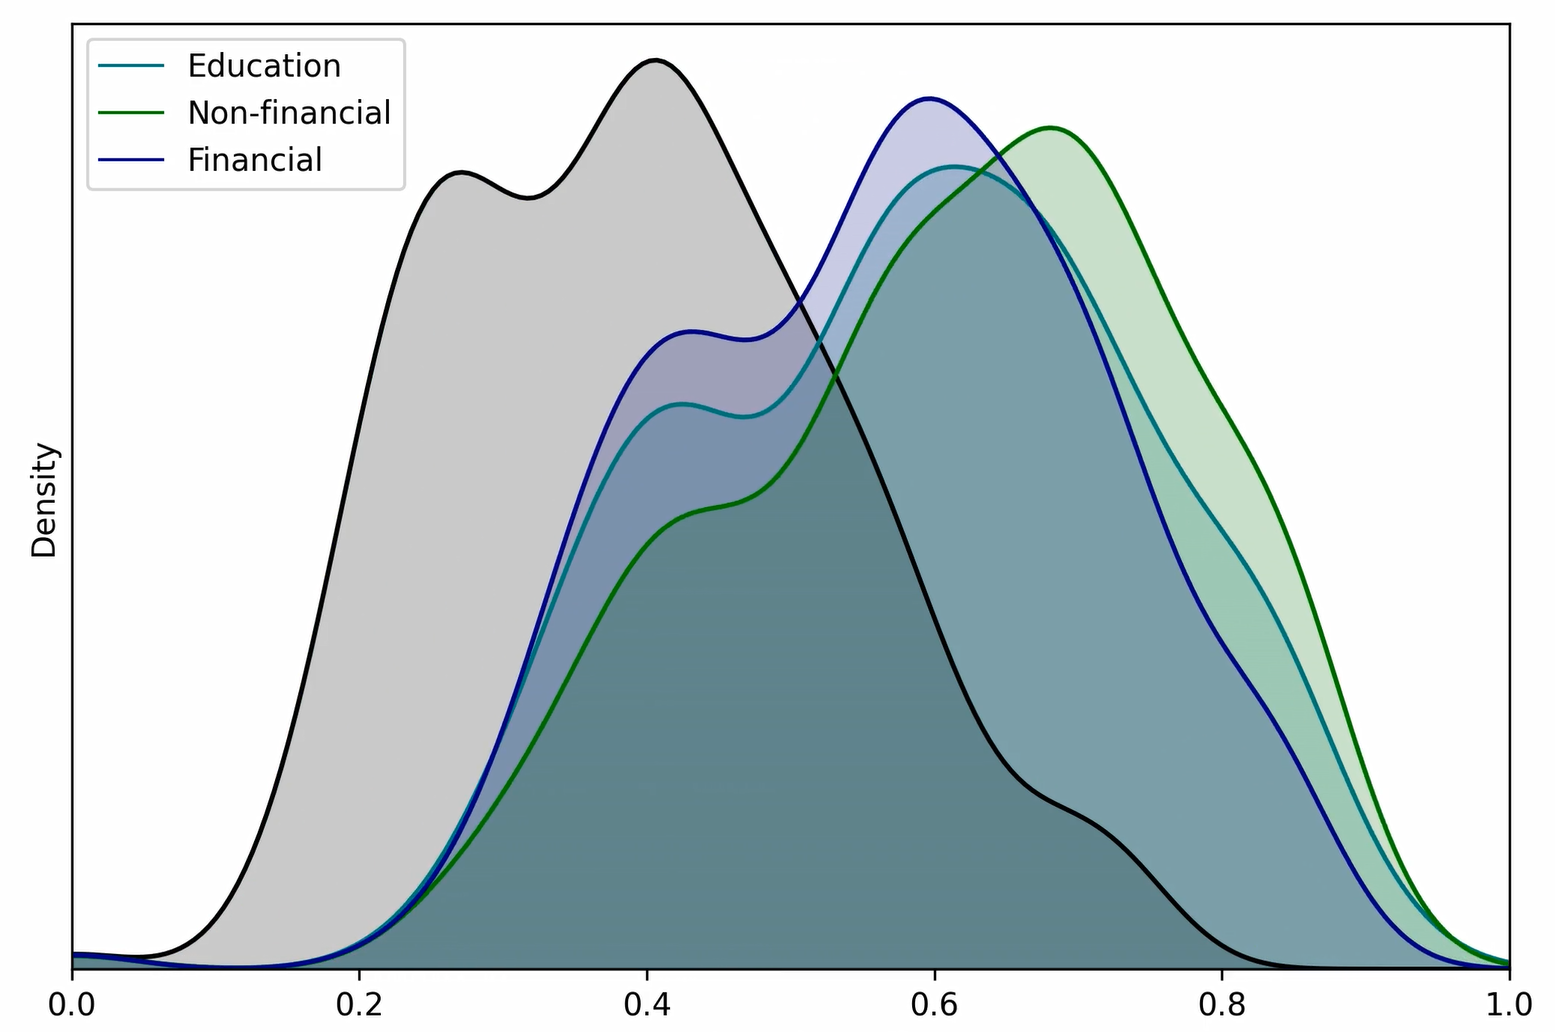
\includegraphics[width=0.99\linewidth]{images/policies.png}
	\end{center}	
\end{frame}

\section{Identification}

\begin{frame}{Simplifying Interference -- Weak Dependence}
	Learning $Y_i(\mathbf{a})$ is difficult
	~\\~\\
	\begin{center}
		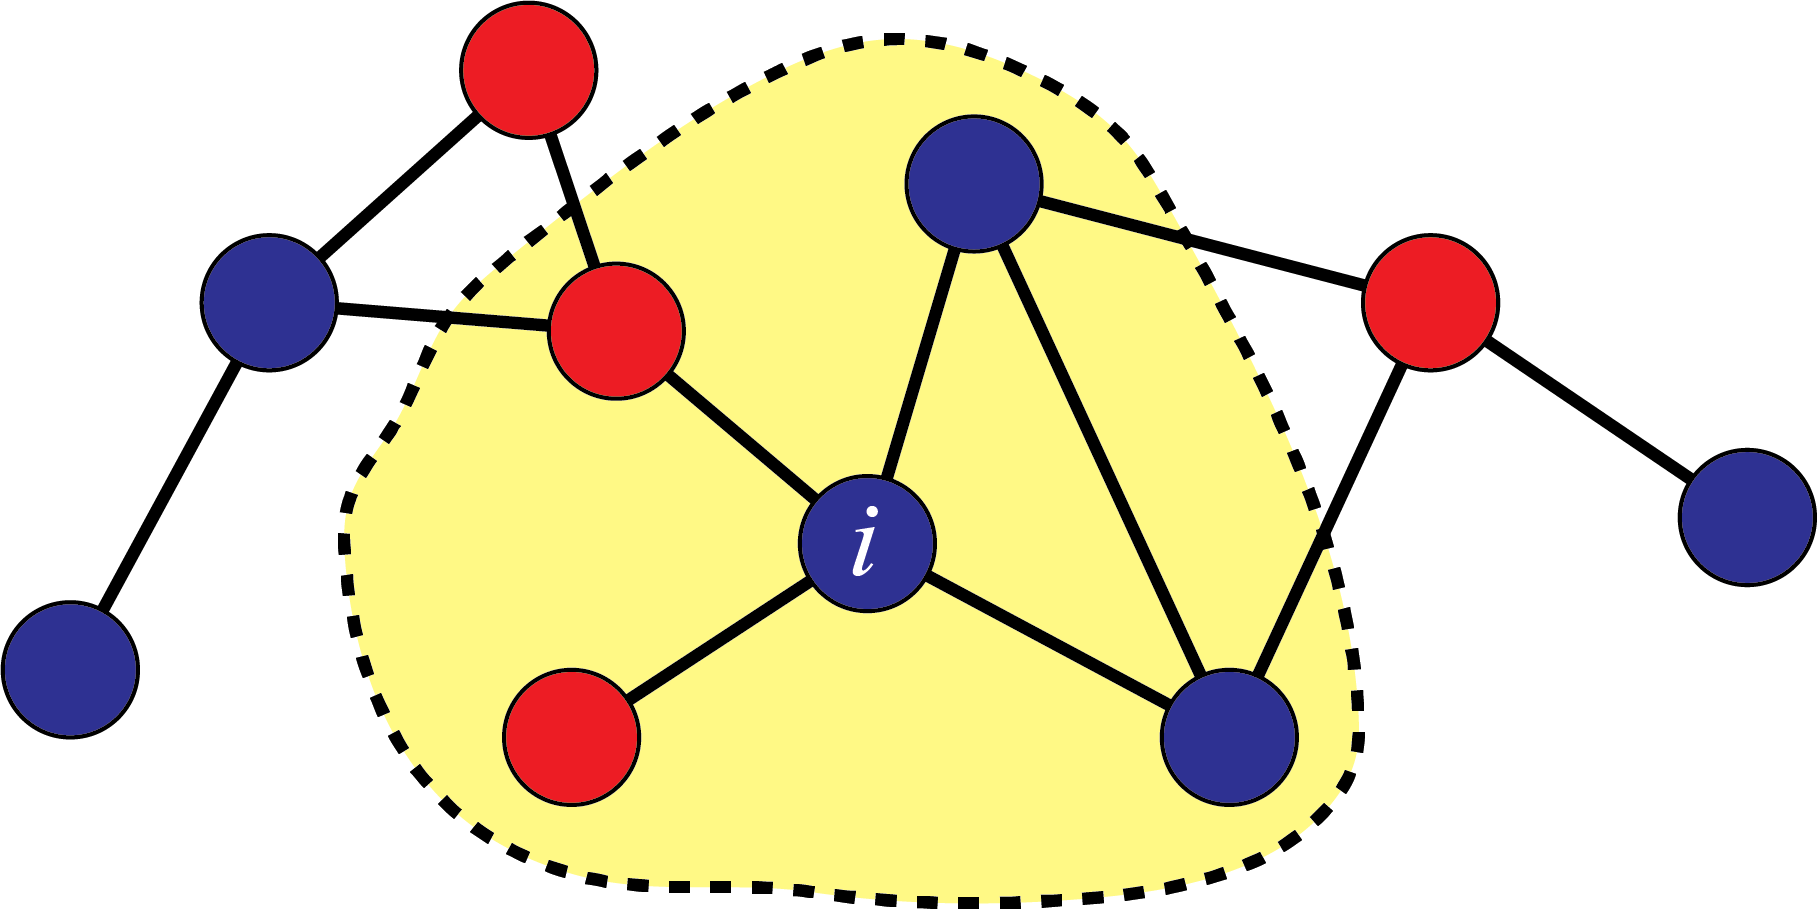
\includegraphics[width=0.90\linewidth]{images/WeakDependence.png}
	\end{center}
\end{frame}

\begin{frame}{Covariate Mappings}
	Rely on a \textit{parametric mapping}
	\begin{equation*}
		Y_i(a_i, a_{-i}) = Y_i(a_i, a_i^s) \ne Y_i(a_i)
	\end{equation*}
	where $a_i^s$ is a parametric map of $i$'s direct contacts
	~\\~\\
	Here $a^s$ denotes a general covariate mapping of direct contacts
	\begin{itemize}
		\item But need to choose something specific\footnote[frame]{These definitions treat all contacts as equivalent but relax via edge weights or multiple edge types}
		\item Assume parametric mapping is correct
	\end{itemize}
\end{frame}

\begin{frame}{Covariate Mapping Examples}
	Count
	\begin{equation*}
		X_i^s := \sum_{j \in n} X_j \mathfrak{G}_{ij}
	\end{equation*}
	Proportion
	\begin{equation*}
		X_i^s := \frac{\sum_{j \in n} X_j \mathfrak{G}_{ij}}{\sum_{j \in n} \mathfrak{G}_{ij}}
	\end{equation*}
	Threshold
	\begin{equation*}
		X_i^s := I \left\{ \left(\sum_{j \in n} X_j \mathfrak{G}_{ij}\right) >= t \right\}
	\end{equation*}
\end{frame}

\begin{frame}{Identification Assumptions}
	\begin{block}{Causal consistency}
		\begin{equation*}
			\text{if } a = A_i, a^s = A_i^s \text{ then } Y_i = Y_i(a_i, a_i^s)
		\end{equation*}
	\end{block}
	\begin{block}{Exchangeability}
		\begin{equation*}
			Y_i(a, a_s) \amalg A_i ,A_i^s \mid W_i, W_i^s
		\end{equation*}
	\end{block}
	\begin{block}{Positivity}
		\begin{align*}
			\text{if } & {\Pr}^*(A=a,A^s=a^s \mid W,W^s) > 0 \text{ then } \\
			& \Pr(A=a,A^s=a^s \mid W,W^s) > 0
		\end{align*}
	\end{block}
\end{frame}

\section{Other Systematic Errors}

\begin{frame}{Missing Data}
	Missing data on vaccination and covariates
	~\\~\\
	Multivariate Imputation with Chained Equations (MICE)
	\begin{itemize}
		\item Modified MICE to include $A^s,W^s$ in models
	\end{itemize}
	~\\
	100 imputed data sets
\end{frame}

\begin{frame}{Measurement Error of Contacts}
	Self-reported contacts are known to be misreported\footnote[frame]{Mastrandrea et al. \textit{PloS ONE} 2015;10(9):e0136497}
	~\\~\\
	 Multiple Imputation for Measurement Error (MIME)
		\begin{itemize}
			\item Bayesian procedure with stochastic block model\footnote[frame]{Young et al. \textit{Journal of Complex Networks} 2021;8(6)}
			\item Sensitivity and specificity informed by Bluetooth data collected on subset of students
		\end{itemize}
	~\\
	100 networks for each imputed data set
	\begin{itemize}
		\item Summarized 10,000 imputations using nested Rubin's Rule
	\end{itemize}
\end{frame}

\section{Estimation}

\begin{frame}{Targeted Maximum Likelihood Estimation (TMLE)}
	TMLE for network dependent data\footnote[frame]{van der Laan \textit{Journal of Causal Inference} 2014;2(1):13-74, Sofrygin \& van der Laan \textit{Journal of Causal Inference} 2017;5(1):20160003, Zivich et al. \textit{Stats in Med} 2022;41(23):4554-4577}
	\begin{itemize}
		\item[1.] Fit nuisance model for $Y \mid A,A^s,W,W^s$
		\item[2.] Fit nuisance model for $A,A^s \mid W,W^s$
		\item[3.] Fit targeting model
		\item[4.] Targeted prediction(s)
		\item[5.] Inference via influence function
	\end{itemize}
\end{frame}

\begin{frame}{Step 1: Outcome Nuisance Model}
	Treat observations as if they are independent and fit a model for\footnote[frame]{This is the g-computation analog for network-dependent data}
	\begin{equation*}
		E[Y \mid A, A^s, W, W^s]
	\end{equation*}
	~\\
	Then generate predicted values from this model, $\hat{Y}$, with $A, A^s$
	~\\~\\
	Here, logistic regression with $L_2$ penalty
\end{frame}

\begin{frame}{Step 2: Action Nuisance Model}
	For the targeting step, need\footnote[frame]{This is the weight for the IPW analog with network-dependent data}
	\begin{equation*}
		\frac{\pi_i^*}{\pi_i} = \frac{{\Pr}^*(A_i = a, A_i^s = a_i^s \mid W_i, W_i^s)}{\Pr(A_i = a, A_i^s = a_i^s \mid W_i, W_i^s)}
	\end{equation*}
	~\\
	Factor $A,A^s$ and model as if independent
	~\\~\\
	Use a Monte Carlo procedure to go from  
	$${\Pr}^*(A_i = a \mid W_i, W_i^s) \rightarrow {\Pr}^*(A_i = a, A_i^s=a^s \mid W_i, W_i^s)$$
	~\\
	Here, logistic regression and Poisson\footnote[frame]{$A^s$ was chosen to be count mapping}
\end{frame}

\begin{frame}{Step 3: Targeting Step}
	Fit the following weighted model
	\begin{equation*}
		\text{logit}\left\{ \Pr(Y_i = 1) \right\} = \eta + \text{logit}(\hat{Y}_i)
	\end{equation*}
	where weights are $\frac{\pi_i^*}{\pi_i}$ from the previous step
\end{frame}

\begin{frame}{Step 4: Interest Parameter}
	Monte Carlo procedure
	\begin{itemize}
		\item[a.] Set actions according to ${\Pr}^*(A_i = a \mid W_i, W_i^s)$.\footnote[frame]{Can simplify by reusing copies from Step 2}
		\item[b.] Compute $\hat{Y}^*$ under $A^*, A^{s*}$.
		\item[c.] Update $\hat{Y}^*$ using $\hat{\eta}$, then take mean.
		\item[d.] Repeat (a.) through (c.) $k$ times.
		\item[e.] Take average of the $k$ different means as $\hat{\psi}$.
	\end{itemize}
\end{frame}

\begin{frame}{Step 5: Inference}
	Influence function variance estimator with latent dependence\footnote[frame]{Dependence up to second-order contacts. Ogburn EL et al. \textit{JASA} 2024;119(545):597-611}
	\begin{equation*}
		\frac{1}{n} \sum_{i=1}^{n} \sum_{j=1}^{n} \left[ \frac{\pi_i^* (\hat{\alpha}, \hat{\gamma})}{\pi_i (\hat{\alpha}, \hat{\gamma})} \left(Y_i - \hat{Y}_i \right) \right] \times \left[\frac{\pi_j^* (\hat{\alpha}, \hat{\gamma})}{\pi_j (\hat{\alpha}, \hat{\gamma})} \left(Y_j - \hat{Y}_j \right)\right] \times \mathbb{G}_{ij}
	\end{equation*}
	\begin{itemize}
		\item where $\mathbb{G}_{ij} = \mathfrak{G}_{ij}$ for $i \ne j$ and $\mathbb{G}_{ij} = 1$ otherwise
	\end{itemize}
\end{frame}

\section{Results}

\begin{frame}{Descriptive Summary}
	\centering
	\begin{tabular}{llc}
		\hline
		&                        & Overall ($n=454$) \\ \cline{3-3} 
		\multicolumn{2}{l}{Influenza-Like Illness}             & 190 (42\%)        \\
		\multicolumn{2}{l}{Laboratory-confirmed} & 17 (4\%)          \\
		\multicolumn{2}{l}{Vaccination}          & 161 (40\%)        \\
		& Missing                & 52 (11\%)         \\ \hline
	\end{tabular}
	~\\~\\~\\~\\
	\begin{tabular}{lc}
		\hline
		& Unvaccinated ($n=241$)             \\ \cline{2-2} 
		Educational         & 50 (11\%)          \\
		Non-financial       & 93 (20\%)          \\
		Financial           & 18 (4\%)           \\
		Contraindication(s) & 2 (\textless{}1\%) \\ \hline
	\end{tabular}
\end{frame}

\begin{frame}{Results}
	\begin{center}
		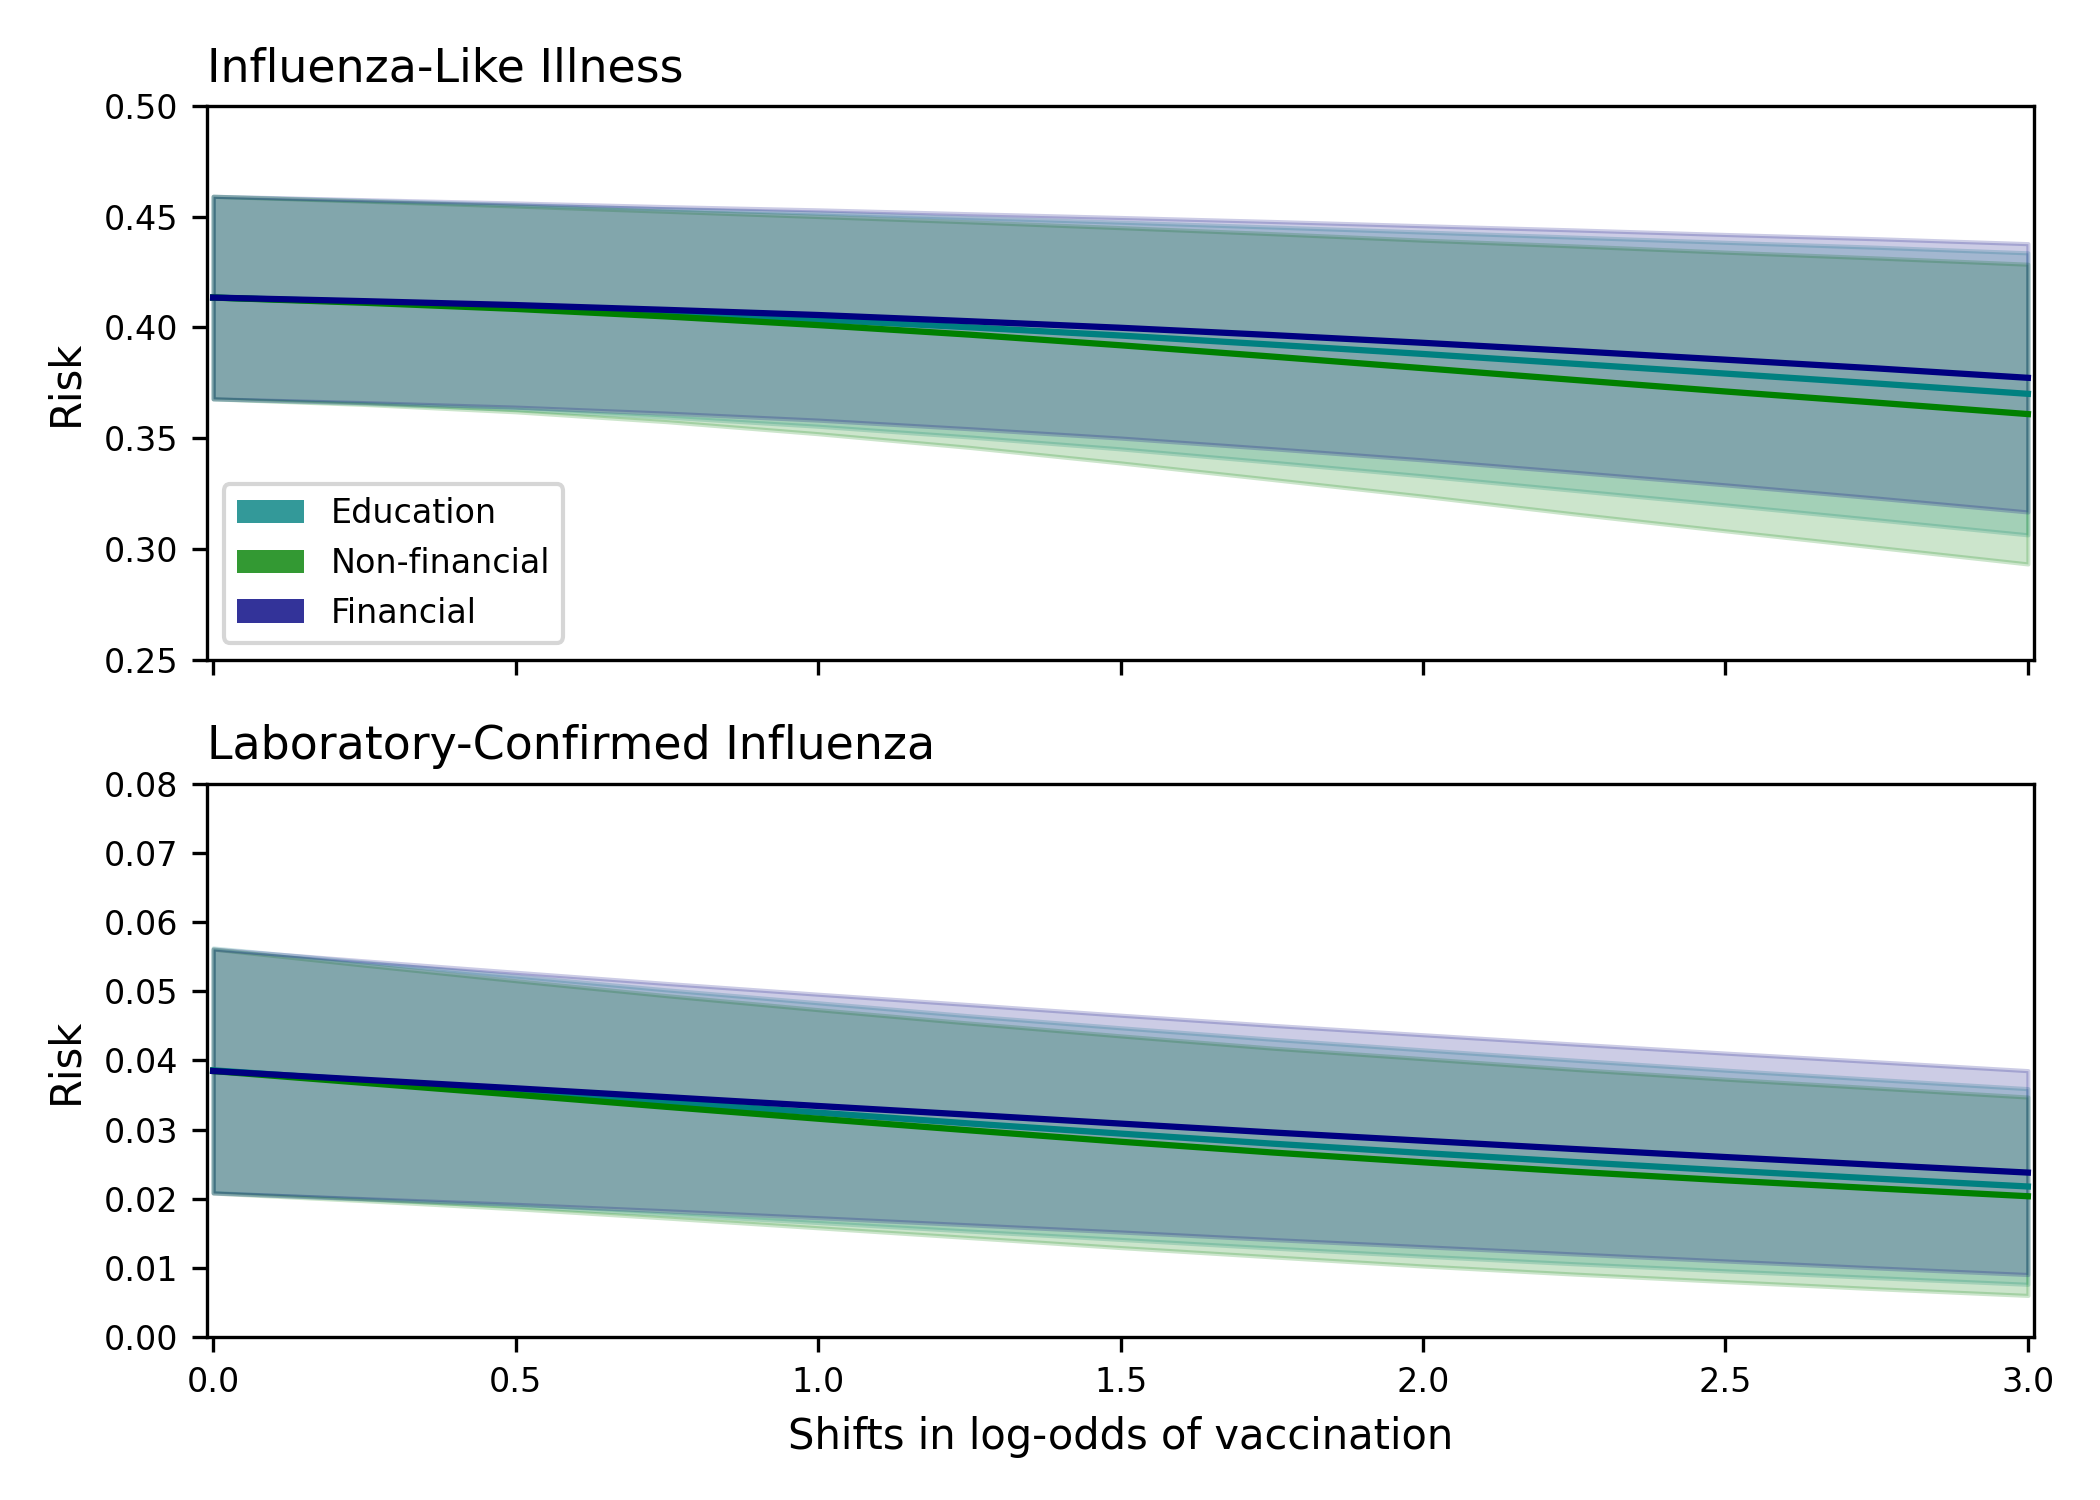
\includegraphics[width=0.99\linewidth]{images/aim3_measure.png}
	\end{center}
\end{frame}

\section{Conclusions}

\begin{frame}{Conclusion}
	Interference is common in epidemiology
	\begin{itemize}
		\item Modifies how we should view parameters
		\item Consider what is meaningful for public health
		\item Need methods (and data) that can accommodate
	\end{itemize}
	~\\
	But there are still many challenges
\end{frame}

\begin{frame}{Practical Challenges}
	\begin{columns}
		\begin{column}{0.5\textwidth}
			Collection of network data
			\begin{itemize}
				\item Measure large networks
				\item Reduce measurement error
			\end{itemize}
			~\\
			Modeling
			\begin{itemize}
				\item Weak dependence
				\item Covariate mappings
			\end{itemize}
		\end{column}
		\begin{column}{0.5\textwidth}
			Missing data
			\begin{itemize}
				\item Dependence between observations
			\end{itemize}
			~\\
			Partially observing network
			~\\~\\
			Inference doesn't incorporate that $\Pr^*$ is based on estimated probabilities
		\end{column}
	\end{columns}
\end{frame}

\begin{frame}{Future Directions}
	Longitudinal Network TMLE
	\begin{itemize}
		\item Weak dependence only in interval
	\end{itemize}
	~\\
	Covariate mappings
	\begin{itemize}
		\item Explore flexible specification approaches
	\end{itemize}
	~\\
	Compare against alternative approaches\footnote[frame]{Tchetgen Tchetgen et al. \textit{JASA}, 2021;116(534):833-844.}
\end{frame}

\begin{frame}{Thank You!}
	\begin{center}
		\LARGE
		Questions?
	\end{center}
	~\\
	\begin{center}
		\small
		\faEnvelope \quad pzivich@unc.edu \qquad \quad 
		\faGithub \quad pzivich \qquad \quad
		pausalz@bsky.social
	\end{center}
\end{frame}

\section{Appendix}

\begin{frame}{Identification in Example}
	Covariates included in $W$
	\begin{itemize}
		\item gender, race, stress (Perceived Stress Scale-10), optimal hand hygiene, high-risk conditions, sleep quality, alcohol use, trial arm, number of unique contacts
	\end{itemize}
	~\\
	Covariate mappings
	\begin{itemize}
		\item Vaccination: count
		\item Gender, race, hand hygiene, high-risk, alcohol use, trial arm: count
		\item stress: variance
	\end{itemize}	
\end{frame}

\begin{frame}{Plans}
	Educational
	\begin{itemize}
		\item Target those: influenza vaccine causes influenza, don't get influenza, didn't know they could get the influenza vaccine
	\end{itemize}
	Non-financial
	\begin{itemize}
		\item Target those: never got around to it, did not have transportation, hours available were inconvenient
	\end{itemize}
	Financial
	\begin{itemize}
		\item Target those: health plan did not cover, no health insurance
	\end{itemize}
\end{frame}

\begin{frame}{Probability Weights Monte Carlo}
	Monte Carlo procedure to get $\pi_i^*$
	\begin{itemize}
		\item[a.] Create copy of data
		\item[b.] Set $A$ according to ${\Pr}^*(A_i = a \mid W_i, W_i^s)$ to get $A^*, A^{s*}$
		\item[c.] Repeat (a.) and (b.) for $k$ copies of data
		\item[d.] Fit models for $\Pr(A_i^* = a, A_i^{s*} = a_i^s \mid W_i, W_i^s)$ using all $k$ copies
		\item[e.] Predict probability using models from (d.) and \textit{observed} $W,W^s,A$
	\end{itemize}
\end{frame}

%\begin{frame}{Parameter of Interest}
%	Simplifying using the previous restrictions on interference
%	\begin{equation*}
%		\psi = \frac{1}{n} \sum_{i=1}^{n} E \left[ \sum_{a,a^s \in \mathcal{A}, \mathcal{A}^s} 	Y_i(a_i, a_i^s) \; {\Pr}^*(A_i = a, A_i^s = a^s \mid W_i, W_i^s) \mid \mathbf{W} \right]
%	\end{equation*}
%\end{frame}


\end{document}